\documentclass[letterpaper,twocolumn,10pt]{article}

\usepackage{hyperref} % For clickable links; need to load this before usenix.
\usepackage{usenix-2020-09}

\usepackage{booktabs} % For nicely-typeset tables.
\usepackage{xspace}
\usepackage{tikz} % For self-contained diagrams.
\usepackage{amsmath} % For the 'align' environment.
\usepackage[scaled=0.8]{beramono} % For a pleasant monospace font.
\usepackage{listings} % For pretty code snippets.
\usepackage{balance} % For balanced references on the last page.
\usepackage{todonotes} % For pretty todos in the paper.
\usepackage{pifont} % For dingbats symbols.


\usepackage[maxbibnames=4, sorting=none]{biblatex} % For more flexible references.

\definecolor{todocolor}{HTML}{FFA0A0}
\newcommand{\phw}[1]{\todo[inline,color = todocolor]{\textbf{Philipp:} #1}\xspace}

%\renewcommand*\familydefault{\ttdefault} % Use Beramono instead of our default monospace font.
\usetikzlibrary[shapes,arrows,positioning,arrows.meta,calc,fit]

\definecolor{darkblue}{rgb}{0,0,0.5}
\hypersetup{
	pdftitle={},
	pdfauthor={},
	pdfkeywords={},
	colorlinks=true,
	urlcolor=darkblue,
	linkcolor=darkblue,
	citecolor=darkblue,
}

\lstset{
    numberstyle=\footnotesize\color{gray},
    basicstyle=\footnotesize\ttfamily,
    stringstyle=\color{Mahogany},
    keywordstyle=\color{MidnightBlue}\bfseries,
    breakatwhitespace=false,
    breaklines=true,
    captionpos=b,
    keepspaces=true,
    numbers=left,
    numbersep=5pt,
    showspaces=false,
    showstringspaces=false,
    showtabs=false,
    tabsize=2
}

\addbibresource{references.bib}

\begin{document}

\title{A Framework for Building Networked Enclaves}

\author{Anonymous}

\maketitle

% As a general rule, do not put math, special symbols or citations
% in the abstract
\begin{abstract}

Enclave deployments often fail to simultaneously be
\emph{secure} (e.g., resistant to side channel attacks),
\emph{powerful} (i.e., as fast as an off-the-shelf server), and
\emph{flexible} (i.e., unconstrained by development hurdles).
%
In this paper, we present \tool{}, an open tool kit that enables the
development of enclave applications that satisfy all three properties.
%
We build \tool{} on top of the recently-proposed AWS Nitro Enclaves whose
architecture prevents side channel attacks by design, making \tool{} more
secure than comparable frameworks.  We abstract away the constrained
development model of Nitro Enclaves, making it possible to run unmodified
applications inside an enclave that have seamless and secure Internet
connectivity, all while making our code user-verifiable.
%
To demonstrate \tool{}'s flexibility, we design three enclave applications, each
a research contribution in its own right:
%
(i) we run a Tor bridge inside an enclave, making it resistant to protocol-level
deanonymization attacks;
%
(ii) we built a service for securely revealing infrastructure configuration,
empowering users to verify privacy promises like the discarding of IP addresses
at the edge;
%
(iii) and we move a Chromium browser into an enclave, thereby isolating its
attack surface from the user's system.

\end{abstract}

\section{Introduction}

% What's the problem that we're trying to solve.
First introduced in 2015, Intel's SGX technology inspired diverse applications
but also increasingly sophisticated attacks: Researchers successfully adapted
speculative execution attacks~\cite{VanBulck2018a}, injected software
faults~\cite{Murdock2020a}, and exploited side channels introduced by shared
caches~\cite{Brasser2017a}, all with the goal of exfiltrating information that
was meant to remain in the enclave.  The underlying flaw that most attacks take
advantage of is that the untrustworthy operating system and the enclave
\emph{share a CPU}, which opens the flood gates for side channel attacks.

% How Nitro Enclaves are better.
In 2020, several cloud providers began offering ``confidential computing''
solutions; Google's is based on SEV~\cite{googlecc} while Microsoft's is based
on SGX~\cite{azurecc}.  Both offerings inherit the attack classes that plague
the respective architectures.  Amazon tread a different path by inventing a new
enclave architecture---called Nitro enclaves---from the ground
up~\cite{nitro-enclaves}.  Nitro enclaves are essentially virtual machine that
run on dedicated CPUs that are not shared with untrustworthy code.  While the
architecture appears promising, Nitro enclaves remain difficult to use:
Documentation is sparse, few applications exist, and enclaves can only interact
with the outside world via a constrained VSOCK interface.  This paper present
the design, implementation, and real-world application of a software framework
that facilitates the development of networked Nitro enclaves.  Key features of
our framework include
(\emph{i}) the ability for enclave code to seamlessly access the Internet;
(\emph{ii}) a design for the horizontal scaling of enclaves by synchronizing
secret key material; and
(\emph{iii}) a reproducible build system and tooling for users to remotely
attest an enclave's authenticity.

% Challenges that we had to overcome.
During the development of our framework, we had to overcome several challenges.
First, Nitro enclaves are meant to be highly constrained environments and
therefore lack a dedicated networking interface.  We designed a mechanism that
allows enclaves to seamlessly send and receive data over the Internet while
maintaining an allow list of destinations, for defense in depth in case of
enclave compromise.
%
Second, the attestation process for Nitro enclaves was not designed to be done
over the Internet.  To assure clients that they are communicating with an
authentic enclave, we had to find a mechanism to bind a TLS session to an
attestation document.
%
Third, we had to devise a reproducible and yet easy-to-use build pipeline that
allows end users---regardless of their operating system---to compile the enclave
application and end up with the exact same image ID as the enclave provider.
%
Fourth, there is no out-of-the-box way for enclaves to scale horizontally while
synchronizing their key material.  We therefore designed a mechanism that allows
enclaves to synchronize their key material.

% Evaluation.
Having overcome the above challenges, we implemented an easy-to-use Go framework
that abstracts away the nuances of working with networked enclaves.  The use of
Go helps keep the trusted computing base small and greatly reduces the risk of
memory corruption bugs.  We show our framework's potential by conducting
performance measurements, and we demonstrate its use and robustness by building
two production-quality applications on top of it; (\emph{i}) an IP address
pseudonymization service, and (\emph{ii}) a $k$-anonymity service that is part
of a privacy-preserving telemetry system.

\paragraph{Contributions}

This work makes three core contributions.
%
First, the design and implementation of a freely available Go framework that
facilitates the implementation and deployment of enclave applications.  The
framework consists of a library that an application can use to run as an
enclave, and tooling that facilitates deterministic builds and seamless
communication with the secure enclave.
%
Second, we make it possible via our framework to turn enclaves into networked
applications.
%
Third, we demonstrate the use of our framework by applying it in three
production-quality code bases; (\emph{i}) in a system that anonymizes client IP
addresses, (\emph{ii}) to run an OPRF service, and to (\emph{iii}) run a server
that's part of a private telemetry system.  We further evaluate our prototypes
with respect to performance and security---especially related to code
complexity.

\paragraph{Structure}

Section~\ref{sec:background} provides background on secure enclaves in general
and AWS Nitro Enclaves in particular.  Section~\ref{sec:design} introduces the
design and implementation of our software framework in addition to the build
process that guarantees reproducible enclave application builds, followed by
Section~\ref{sec:applications} which presents three production-quality
applications that are built on top of our framework.  We measure our framework's
networking performance in Section~\ref{sec:evaluation} and discuss its
limitations in Section~\ref{sec:limitations}.  Finally,
Section~\ref{sec:related-work} constrasts our work with past research.

\section{Background}%
\label{sec:background}

We begin by providing an overview of secure enclaves in general
(\S~\ref{sec:enclaves}), followed by the AWS Nitro system (\S~\ref{sec:nitro})
and Nitro enclaves (\S~\ref{sec:nitro-enclaves}).  We finally compare Nitro
enclaves to SGX-based enclaves (\S~\ref{sec:comparison}).

\subsection{Secure enclaves}%
\label{sec:enclaves}

Computers operate on data that is at rest, in transit, and in use.  We have
well-understood and practical ways to protect data at rest (e.g., full disk
encryption) and in transit (e.g., TLS) but only limited solutions for data that
is in use.  Cryptography provides solutions in the form of fully homomorphic
encryption (FHE) and secure multiparty computation (MPC) but for many
applications, those building blocks remain too slow and cumbersome.  Trusted
execution environments---in particular in the form of ``secure
enclaves''---provide an alternative that is rooted in hardware and code.  Unlike
FHE and MPC, enclaves perform at native (or near-native) execution speed because
they are general-purpose computing environments that are not limited to the
computation of carefully designed functions.  Conceptually, enclaves are
isolated execution environments that are shielded off from a computer's main
execution environment, which runs the untrustworthy (from the enclave's point of
view) operating system.  Enclaves offer various security properties but in the
context of this work, we rely on the following three:

\begin{description}
  \item[Confidentiality] An unauthorized entity (e.g., the operating system)
    must not be able to observe the data that an enclave is processing.

  \item[Integrity] An unauthorized entity must not be able to modify the data
    that the enclave is processing, or the code that it is running.

  \item[Verifiability] A separate entity (e.g., an end user) must be able to
    verify if the enclave is running the code that its operator claims it is
    running.
\end{description}

Major hardware vendors offer CPUs that implement secure enclaves: Intel has SGX,
ARM has TrustZone, and AMD has SEV.  A frequent critique of these industry
efforts focuses on their proprietary nature. The community has a conceptual
understanding of the mechanisms behind enclaves but their exact hardware
implementation is not disclosed, which served as motivation towards an open
source enclave~\cite{Lee20a}.  In practice, enclaves promise to be useful in
situations where a system must process sensitive data while simultaneously be
shielded off from the complexity (and subsequent insecurity) of general-purpose
computers.

\subsection{The AWS Nitro system}%
\label{sec:nitro}

Nitro enclaves are virtual machines that run on dedicated hardware that is not
shared with an enclave's EC2 host.  The technology that enforces isolation
between the enclave and its EC2 host also enforces isolation between any two
given EC2 instances: the Nitro system.  Before covering enclaves, we explain how
the Nitro system works---first by discussing its three key components.

\emph{Nitro cards}: While physically connected to a server's main board via
PCIe, Nitro cards are dedicated and custom-built hardware and software that runs
independently of a server's main board.  Nitro cards implement the interfaces
that allow for the management of a server's computational, memory, and storage
needs, among other things.  A Nitro card also provides a server's hardware root
of trust and is responsible for firmware updates, secure boot, and acts as an
interface between the server and the EC2 control plane.~\cite[pp.
7--10]{Bean2022a}.

\emph{Nitro security chip}: The Nitro card acts independently of the system main
board.  The purpose of the Nitro security chip, which is controlled by the Nitro
card, is to extend the Nitro card's control over the system main board.  One of
the chip's responsibilities is to prevent the CPU from updating the system's
firmware when run in bare metal mode~\cite[pp.~10--11]{Bean2022a}.

\emph{Nitro hypervisor}:
The hypervisor is a firmware-like component that receives command from the Nitro
card.  The hypervisor is stripped of any non-essential code: it does not contain
networking code, file systems, shells, or other utilities that would allow a
successful attacker to access other infrastructure~\cite[pp.~11--12]{Bean2022a}.
%  - kvm-based
%  - custom MM
%  - awaits commands from nitro controller
%  - not connected to the network
%  - no dom0

Other design decisions are meant to provide defense in depth: (i) By
design, the Nitro system has no operator access, i.e., operators are unable to
log in to an EC2 Nitro system and inspect memory or access customer
data~\cite[p.~15]{Bean2022a}. (ii) The Nitro system is designed to communicate
passively, i.e., system components never initiate outgoing connections during
production operations.

Of particular interest is how the Nitro system aims to prevent side channel
attacks: customer instances never share a given CPU core in parallel.  If two
customers use a CPU core sequentially, the hypervisor ensures that state is
cleared in between use.  Depending on the instance, cores may be exclusively
allocated to a customer, which includes Nitro enclaves.  That means that L1 and
L2 caches are also never shared.  Last-level cache lines may be shared but only
non-simultaneously.  Amazon's documentation further
states~\cite[p.~19]{Bean2022a}:

\begin{quote}
By virtue of its function, only relatively infrequently accessed data is
referenced in last-level cache lines.  Side-channels typically require a very
large and statistically relevant number of samples in order to over-come the
noise present in systems.
\end{quote}

\subsection{Nitro enclaves}%
\label{sec:nitro-enclaves}

Nitro enclaves inherit the isolation and security properties of the Nitro
system.  When an EC2 host system launches a Nitro enclave, it ``sacrifices'' at
least one of its CPUs and some of its memory pages to the enclave.  These
resources are subsequently unavailable to the EC2 host and exclusively used by
the enclave.  The same isolation mechanism that protects individual customer EC2
instances from each other also protects the Nitro enclave from its host.

\begin{figure}[t]
  \centering
  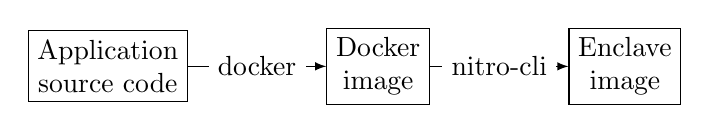
\begin{tikzpicture}[node distance=20pt]

  \node [draw,
         align=center] (code) {Application\\source code};

  \node [draw,
         align=center,
         right=50pt of code] (docker) {Docker\\image};

  \node [draw,
         align=center,
         right=50pt of docker] (eif) {Enclave\\image};

  \draw[-latex] (code.east) -- (docker.west)
                node [midway, fill=white] {docker};
  \draw[-latex] (docker.east) -- (eif.west)
                node [midway, fill=white] {nitro-cli};

\end{tikzpicture}

  \caption{The development workflow for compiling enclave applications.
  Docker's command line tool compiles application source code into a Docker
  image, which is then compiled to an enclave image file using the nitro-cli
  command line tool.}\label{fig:dev-workflow}
\end{figure}

On the software level, Nitro enclaves are virtual machines.  They have their own
Linux kernel that is independent from the host.  Customers can create enclave
images from a Docker image that contains the enclave application.  Amazon
provides a command line tool, nitro-cli~\cite{nitro-cli}, which compiles a
Docker image into an enclave image file (EIF).  Figure~\ref{fig:dev-workflow}
illustrates the process.  As part of compilation, nitro-cli prints a number of
platform configuration registers (PCRs) that contain SHA-384 hashes over
distinct layers of the enclave image file.  Table~\ref{tab:pcr} shows the six
available PCRs.  PCR0 is of particular importance for remote attestation as we
will explain later.

\begin{table}[t]
    \centering
    \begin{tabular}{r l}
    \toprule
      PCR \# & SHA-384 hash of\ldots \\
    \midrule
      0 & Enclave image file \\
      1 & Linux kernel \\
      2 & Application \\
      3 & IAM role assigned to the host instance \\
      4 & Instance ID of the host instance \\
      8 & Enclave image file signing certificate \\
    \bottomrule
    \end{tabular}
    \caption{The available platform configuration registers (PCRs) and the
    meaning behind them.}\label{tab:pcr}
\end{table}

By design, Nitro enclaves have very limited abilities to communicate with the
outside world.  Lacking a dedicated networking interface, Nitro enclaves can
only communicate with their EC2 host via a VSOCK interface~\cite{vsock}.
Originally proposed for communication between a hypervisor and its virtual
machines, AWS repurposed the VSOCK interface to serve as communication channel
between an enclave and its parent EC2 instance.  From a developer's point of
view, the VSOCK interface is a point-to-point interface connecting the two.  On
the address layer, 32-bit context IDs take the role of IP addresses in VSOCK
interfaces.  For example, the enclave may have context ID 4 while its parent EC2
instance may have context ID 3.  On the transport layer, one can use the same
protocols that one can use over the IP-based address family; namely TCP, UDP,
etc.

\subsection{Nitro enclaves versus SGX}%
\label{sec:comparison}

We now make an attempt to compare how Nitro enclaves and SGX differ in their
threat model, their development model, and in the way they can address security
vulnerabilities.

% Hard to get authoritative information on SGX TCB and threat model.  Some
% decent (yet incomplete) information:
% https://people.csail.mit.edu/alinush/6.858-fall-2014/2015/l08-sgx.html
% https://community.intel.com/t5/Intel-Software-Guard-Extensions/SGX-threat-Model/m-p/1187359
\emph{Threat model}:
Both Nitro enclaves and SGX protect against compromise of the host operating
system.  SGX further protects against compromise of any component other than the
CPU itself, which includes---if present---the hypervisor.  Specifically, SGX
assumes that there are no flaws in the CPU's silicon or microcode, and the
private key is not compromised.  While not explicitly stated, Amazon's design
document suggests that Nitro enclaves assume that the Nitro system (including
the Nitro card, the security chip, and the hypervisor) is trusted.  Both Nitro
enclaves and SGX assume that side channel attacks are not feasible.  For SGX,
this assumption has not held~\cite{Nilsson20a,Fei2021a}.

\emph{Development}:
Intel's SGX was not designed to seamlessly move entire applications into the
context of an enclave because the libc that is provided by Intel's SDK lacks
support for many functions and system calls.  Instead, application developers
were meant to partition their application, i.e., move trusted code fragments
into the enclave while the remaining code ran outside the enclave.  However,
projects like Haven~\cite{Baumann2014a} and SCONE~\cite{Arnautov2016a} made it
possible to run entire unmodified applications inside an SGX enclave.  Nitro
enclaves in contrast provide by default what Arnautov et al.\ developed in their
OSDI'14 paper~\cite{Arnautov2016a}: a way to seamlessly run a Docker container
inside an enclave.

\emph{Addressing vulnerabilities}:
What means do Intel and Amazon have to mitigate attacks against their enclave
technology?  Amazon is in possession and control of all hardware and software.
A hardware flaw in Nitro cards may prove expensive and complicated to fix but a
fix is feasible without involving the customer.  Intel has less flexibility
considering that their CPUs are under customer control.  Some SGX
vulnerabilities have been addressed by updating CPU microcode, which may be a
standard procedure for service providers but less so for end users.

\section{Framework Design}
\label{sec:design}

We start by laying out the involved parties and their respective trust
assumptions (\S~\ref{sec:trust-assumptions}), followed by an overview of our
system (\S~\ref{sec:overview}).  We then discuss the two major aspects of our
framework: the build system (\S~\ref{sec:build-system}) and the framework
(\S~\ref{sec:framework}).

\subsection{Trust Assumptions}
\label{sec:trust-assumptions}

Our setting has four participants that have the following trust assumptions:

\begin{enumerate}
    \item The \emph{service provider} wants to process sensitive client
      information.

    \item The \emph{client} is a user of the service provider.  It does not
      trust the service provider and wants verifiable guarantees that the
      service provider will never see the client's sensitive information in
      plain text.  Clients further have an incentive to commit fraud and lie
      about their IP addresses.

    \item The \emph{infrastructure provider} is a third party that provides
      infrastructure to the service provider.  The client trusts that the
      infrastructure provider and the service provider don't collude.

    \item The \emph{enclave provider} makes available enclaves to the service
      provider.  Both the client and the service provider trust that the
      enclave provider's enclaves have the security attributes of integrity,
      confidentiality, and attestability.  The client trusts that the enclave
      provider and service provider don't collude.
\end{enumerate}

\subsection{Overview}
\label{sec:overview}

We begin with a short, informal overview of our system to provide intuition.
The subsequent sections are going to elaborate on this high-level picture.  

\begin{enumerate}
    \item The service provider implements a new service with the intention of
      running it in an enclave.  Once the implementation is finished, the
      service provider publishes the source code for the clients to audit, and
      runs the code in an enclave.  After booting, the enclave obtains a
      CA-signed certificate.

    \item Users audit the source code.  Once a user has convinced herself that
      the code is free of bugs, she compiles the code using the framework's
      deterministic build system, resulting in an image checksum.

    \item The client establishes an end-to-end encrypted network connection to
      the enclave.  Right \emph{after} establishing the connection but
      \emph{before} revealing any sensitive information, the client provides a
      nonce and asks the enclave for an attestation document.

    \item The enclave receives the nonce and asks its hypervisor to generate an
      attestation document that should contain the client-provided nonce
      \emph{and} the fingerprint of the enclave's CA-signed certificate.  The
      resulting attestation document is returned to the client.

    \item The client performs various checks (see \S~\ref{sec:attestation} for
      details) and trusts the enclave if all checks pass.  The client is then
      convinced that it's communicating with the code that the user audited in
      the previous steps, and is willing to reveal her sensitive information to
      the enclave.
\end{enumerate}

% As illustrated in Figure~\ref{fig:overview}, clients submit their IP address
% to the enclave, which is run by the enclave provider but its code comes from
% the service provider.  It's not possible to talk to the enclave directly
% because all communication happens via the (untrustworthy) parent EC2
% instance, which is why we introduce a TCP proxy (run by the infrastructure
% provider), which prevents the EC2 instance from seeing the client's IP
% address.  The client establishes a TLS session that is terminated inside the
% enclave and can therefore be sure that its IP address is sent to the enclave,
% and the enclave only.

% After the enclave received the client's address, it responds with a nonce.
% The enclave does not know if the client reported its real address or a fake
% address, so it must actively verify the address, but it cannot connect to the
% client directly because that would allow the EC2 instance to see the client's
% IP address.  To solve this problem, we make the enclave talk to the client
% via a VPN node.  Upon connection establishment, the client must send the
% nonce it received from the enclave in the previous step.  Once the enclave
% recognizes the nonce, it rests assured that the client really does control
% the IP address it submitted earlier.

% In the final step, the enclave anonymizes the client's IP address and
% forwards it to its back end.

\subsection{The Reproducible Build System}
\label{sec:build-system}

% Why it's not a big deal that only some users can audit our code.
Only a small subset of the users will be skilled enough programmers to audit
the enclave's code for bugs.  We expect non-technical users to trust that other
users---or perhaps professional code audit companies---have studied the code
and pointed out potential bugs.  Once a user has convinced herself of the code's
correctness, she compiles the code to arrive at an image ID.  Crucially, we
need a \emph{deterministic mapping} between the code and its corresponding
image ID because the service provider and clients must agree on the image ID
that's running in the enclave.

Docker does not offer a deterministic mapping because, among other things,
Docker uses timestamps in its build process, causing subsequent builds of
identical code to result in different image IDs.\footnote{In essence, an image
is simply a file system.  If an image is reproducible, separate build processes
arrive at the exact same file system.}  To obtain reproducible builds, we use
the tool kaniko~\cite{kaniko}.  Kaniko's main purpose is to build container
images from a Dockerfile while itself in a container, but we use kaniko because
it can do so reproducibly.  As long as the client and service provider use the
same enclave source code, Go version, and kaniko version, they can build
identical images---even when compiling the code on different platforms, like
Mac OS and Linux.  Equipped with a locally-compiled container image ID, the
client is now ready to interact with the enclave.

\subsection{Framework Features}
\label{sec:framework}

Having established how one can build applications reproducibly, we now turn to
the specific features of our framework.  The following sections discuss how the
framework communicates with the outside world (\S~\ref{sec:networking});
how it seeds its entropy pool, (\S~\ref{sec:entropy});
how it obtains a CA-signed certificate (\S~\ref{sec:cert});
how we facilitate remote attestation (\S~\ref{sec:attestation});
and how enclaves can share their key material to allow for horizontal scaling (\S~\ref{sec:sync});
and finally how to thwart side-channel attacks (\S~\ref{sec:side-channels}).

\phw{Add subsection on an endpoint that allows for the ingestion of
well-defined, private data (e.g., IP address filter lists).}

\subsubsection{Enabling Networking}
\label{sec:networking}

Recall from Section~\ref{sec:nitro} that Nitro enclaves have no dedicated
network interface and are only able to communicate with their respective EC2
host.  Our framework therefore needs to provide code that runs on the parent
EC2 host and forwards packets between clients and the enclave.
Figure~\ref{fig:networking} illustrates our networking architecture.

When the enclave first starts, it fetches a CA-signed certificate from Let's
Encrypt.  To do so, it first connects to Let's Encrypt's infrastructure via a
SOCKS proxy.  Let's Encrypt does not publish its endpoints' IP addresses, which
is why we cannot use point-to-point connections and have to rely on the
flexibility of a SOCKS proxy.\footnote{We implemented both the SOCKS proxy and
the TCP proxy, and make both available under a free license.}

Clients establish end-to-end encrypted TLS sessions with the enclave via a TCP
proxy on the EC2 machine that translates between AF\_INET and AF\_VSOCK.  Note
that the EC2 machine only sees encrypted data. Clients should further only
connect to the EC2 machine via a third party reverse proxy, which also hides
the client's network identity from the EC2 machine.

In case of a compromise, we don't want the application to be able to leak data
to an attacker-controlled endpoint via the SOCKS proxy, which is why we use an
allow list on the SOCKS proxy.  In a typical application, the allow list
consists of two endpoints:

\begin{enumerate}
    \item The domain name acme-v02.api.letsencrypt.org to interact with Let's
      Encrypt.
    \item The IP address of whatever back end machine the enclave needs to talk
      to.
\end{enumerate}


\newcommand{\addr}[1]{{\footnotesize \color{gray}#1 }}

\begin{figure}[t]
\centering
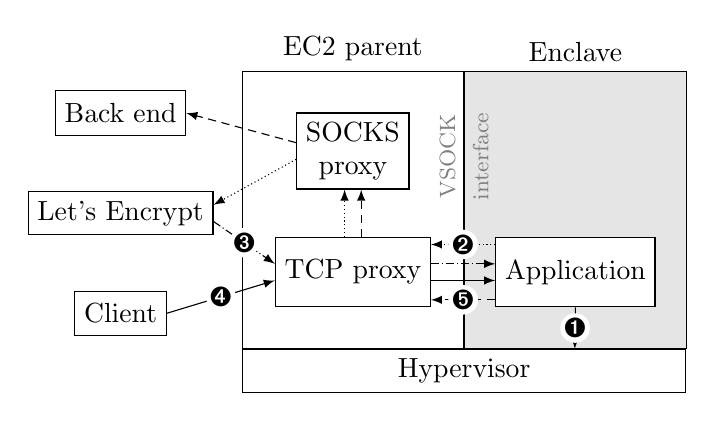
\begin{tikzpicture}[node distance=20pt]
	\node [draw,
           label=EC2 parent,
           minimum height=100pt,
           align=center,
           minimum width=80pt] (ec2) {};
	\node [draw,
           label=Enclave,
           right=0pt of ec2,
           fill=black!10,
           minimum height=100pt,
           minimum width=80pt] (enclave) {};
           
    \node [draw,
           below=0pt of enclave.south west,
           minimum width=160pt] (hypervisor) {Hypervisor};
	   
	\node [draw,
           align=center,
           minimum height=25pt,
           yshift=-5pt,
           above=of ec2.south] (viproxy) {TCP proxy};

	\node [draw,
           align=center,
           yshift=5pt,
           below=of ec2.north] (socks) {SOCKS\\proxy};
  
	\node[draw,
          align=center,
          fill=white,
          minimum height=25pt,
          yshift=-5pt,
          above=of enclave.south] (app) {Application};
	      
	\node [draw,
           minimum height=16pt,
           yshift=35pt,
           left=of ec2.west] (backend) {Back end};

    \node [draw,
           below=of backend] (letsencrypt) {Let's Encrypt};

    \node [draw,
           below=of letsencrypt,
           minimum height=16pt] (client) {Client};

    \node [right, align=center, rotate=90] at (enclave.west) {\footnotesize \color{gray} VSOCK\\\footnotesize \color{gray} interface};

    % Application asks the hypervisor for randomness.
    \draw[-latex] (app.south) -- ([xshift=40pt]hypervisor.north)
        node [midway, fill=white, circle, inner sep=0pt] {\ding{202}};

    % Application talking to Let's Encrypt.
    \draw[-latex, densely dotted] ([yshift=10pt]app.west) -- ([yshift=10pt]viproxy.east)
        node [midway, fill=white, circle, inner sep=0pt] {\ding{203}};
    \draw[-latex, densely dotted] ([xshift=-3pt]viproxy.north) -- ([xshift=-3pt]socks.south);
    \draw[-latex, densely dotted] ([yshift=-3pt]socks.west) -- ([yshift=3pt]letsencrypt.east);

    % Let's encrypt probing Application.
    \draw[-latex, densely dashdotted] ([yshift=-3pt]letsencrypt.east) -- ([yshift=3pt]viproxy.west)
        node [midway, fill=white, circle, inner sep=0pt] {\ding{204}};
    \draw[-latex, densely dashdotted] ([yshift=3pt]viproxy.east) -- ([yshift=3pt]app.west);

    % Clients talking to the application.
    \draw[-latex] (client.east) -- ([yshift=-3pt]viproxy.west)
        node [midway, fill=white, circle, inner sep=0pt] {\ding{205}};
    \draw[-latex] ([yshift=-3pt]viproxy.east) -- ([yshift=-3pt]app.west);
    
    % Application talking to backend.
	\draw[-latex, densely dashed] ([yshift=-10pt]app.west) -- ([yshift=-10pt]viproxy.east)
	    node [midway, fill=white, circle, inner sep=0pt] {\ding{206}};
	\draw[-latex, densely dashed] ([xshift=3pt]viproxy.north) -- ([xshift=3pt]socks.south);
	\draw[-latex, densely dashed] ([yshift=3pt]socks.west) -- (backend.east);
\end{tikzpicture}
\caption{Upon bootstrapping, the application first asks the hypervisor for
  randomness to seed its entropy pool (\ding{202}), followed by initiating an
  ACME session to obtain a Let's Encrypt-signed certificate (\ding{203}), after
  which Let's Encrypt probes the enclave an issues the certificate
  (\ding{204}).  Afterwards, clients can establish HTTPS connections with the
  enclave (\ding{205}) and the enclave can forward data to its back end
  (\ding{206}).  All of the application's ingress and egress  traffic is routed
  over a TCP proxy that translates between AF\_INET and AF\_VSOCK.  Egress
  traffic is reaches the Internet via a SOCKS proxy.}
\label{fig:networking}
\end{figure}

\subsubsection{Seeding the Entropy Pool}
\label{sec:entropy}

Like virtual machines, a Nitro secure enclave is an entropy-starved, sterile
environment that lacks access to periphery devices that could help the kernel
seed its entropy pool.  To work around that, the Nitro's hypervisor can provide
randomness that the enclave can use to seed its entropy pool.  Our framework
automatically takes advantage of that when it first starts, so application
developers are never going to run into function calls that block because of a
lack of randomness.

\subsubsection{End-to-end Secure Channel}
\label{sec:cert}

Having established how the enclave can send and receive network packets, we now
turn our attention to secure channels.  More specifically: how can a host on
the Internet be sure that it's talking to the enclave application code it
audited, without taking advantage of an existing trust relationship?

We implement a secure channel based on HTTPS.  Once the enclave initialized its
entropy pool, it obtains an HTTPS certificate that allows clients to establish
end-to-end encrypted session with the enclave.  Crucially, the HTTPS
certificate \emph{lives and dies} inside the enclave and its private key cannot
be extracted (or injected) by the service provider.  Our framework allows for
the creation of a self-signed certificate or a CA-signed certificate.  If a
self-signed certificate is desired, the framework creates and signs a
certificate for a given FQDN.  To get a CA-signed certificate, the framework
uses Let's Encrypt's ACME protocol because it allows for the generation of a
certificate with no human interaction.  In that case, the enclave initiates an
HTTP-01 challenge connection with Let's Encrypt's infrastructure via our SOCKS
proxy (cf. Figure~\ref{fig:networking}), and subsequently expects an incoming
connection from Let's Encrypt to port 80, which the hosting EC2 image forwards
to the enclave.  Note that the hosting EC2 machine could also obtain a valid
CA-signed certificate for the same FQDN because the enclave and the EC2 image
share a single IP address.  However, this is of little use to the EC2 machine
as we will discuss in the next section.

The application can register arbitrary handlers.

\phw{Explain why we're not using AWS ACM.}

\subsubsection{Remote Attestation}
\label{sec:attestation}

By default, Nitro Enclaves only allow for local attestation.

we could have also dont it via certificate extension~\cite[\S~3.2]{Knauth2019a}

After the client establishes an HTTPS connection with the enclave, it needs to
know that (\emph{i}) the TLS connection it just established is terminated
inside the enclave (instead of by the EC2 machine) and (\emph{ii}) the enclave
is running the code that the user audited in the previous step.  To that end,
the client requests the enclave's \emph{attestation document}---a
hypervisor-signed document that attests to the container image ID that the
enclave is running.  To request an attestation document, the client provides a
\emph{nonce}---a 20-byte random value---whose purpose is to prevent the service
provider from replaying attestation documents.  Phrased differently, the client
provides a nonce to convince itself that it's talking to an live enclave.  In
particular, clients make the following HTTP request to request an attestation
document:

\begin{lstlisting}
GET /attestation?nonce=80835718840fa8652364e8b5d05a9c03d42123b7 HTTP/1.1
\end{lstlisting}

The enclave receives the request and the provided nonce, asks the hypervisor to
include the nonce \emph{and} the fingerprint of the enclave's X.509 certificate
in the attestation document, and sends the resulting attestation document to
the client.  By asking the hypervisor to include the certificate fingerprint in
the attestation document, we effectively bind a TLS session to an enclave.  The
client then verifies the following in order:

\begin{enumerate}
    \item The attestation document is signed by the AWS PKI whose public key is
      known to all parties.
    \item The challenge is part of the attestation document.
    \item The fingerprint of the enclave's X.509 certificate is part of the
      attestation document.
    \item The enclave's image ID is identical to the image ID that the client
      compiled locally.
\end{enumerate}

If all four conditions hold, the client is convinced that it's talking to an
enclave that runs the code that the client audited in the previous step, and
that the TLS connection is terminated in the enclave.  Note that the hosting
EC2 machine is able to intercept HTTPS connections with its own, CA-signed
certificate but clients will only trust the EC2 machine if (and only if) it can
produce an attestation document as expected by the client, which it can't.  Now
that the client has established a trust relationship with the enclave, it's
ready to send sensitive information to the enclave.

While attestation documents can be generated quickly and in rapid
succession---we present performance measurements in
Section~\ref{sec:attestation-performance}, they do require an extra round trip
between the client and the enclave before the client is willing to reveal
sensitive information.  To eliminate that round trip, clients should use TLS
session resumption once they have verified the enclave's attestation document.
The service provider is unable to tamper with the enclave's key material, so
it's safe to re-use a once-established TLS session to forego an unnecessary
round trip.

\paragraph{Client-side Verification}

Even for developers, remote attestation is a complex process that is difficult
to understand and work with, and in our setting, end users are expected to
conduct remote attestation.  We therefore made a careful effort to abstract
away technical details.  A user wishing to remotely attest an enclave
essentially asks herself ``Does the enclave that's exposed at a given URL run
the source code that I just audited?''  We built a tool set that reduces the
process to the running of a Makefile, e.g.:

\begin{lstlisting}
$ make verify CODE="/path/to/enclave/code/" \
              ENCLAVE="https://example.com/attest"
\end{lstlisting}

The first environment variable, \texttt{CODE}, points to the directory
containing the source code that the enclave is supposedly running, and the user
audited.  The second variable, \texttt{ENCLAVE}, points to the URL endpoint of
the enclave that the user's client is connecting to.  When the user runs this
command, the Makefile deterministically compiles the given source code to
obtain its image ID, asks the enclave for an attestation document, verifies the
document, and ensures that the attestation document is for the image ID that
was compiled in the first step.  If all checks pass, the tool informs the user
accordingly.

\subsubsection{Sharing Key Material}
\label{sec:sync}

Compare to \cite{Chen2022a}.

Recall that enclaves are essentially sealed black boxes at runtime, preventing
anyone (including Amazon) from extracting key material that was generated
inside the enclave.  While this is a desirable property, it complicates
horizontal scaling.  If a single enclave is unable to handle the service
provider's traffic load, one must scale horizontally, by starting new enclaves.
In some use cases, it is unacceptable for each enclave to maintain its own key
material.  Instead, enclaves must synchronize their key material, so they
appear to the outside world like a single machine.

While it is possible to build key synchronization using AWS tools like the key
management service (KMS),\footnote{One could encrypt the keys using a KMS
policy that dictates that only enclaves are allowed to decrypt it, and store
the encrypted key in a location that all enclaves can access, e.g., an S3
bucket.} we refrain from using these tools because there is no straightforward
way for users to audit the correct use of these tools.  We therefore devise a
new protocol that enables key synchronization without having to rely on any
extra services.

We solve this problem in two steps: \emph{discovery} and
\emph{synchronization}.  First, enclaves must be able to discover each other,
i.e., learn each other's IP addresses.  Then, enclaves can establish
connections to each other and initiate key synchronization.  Our protocol
dictates that when a new enclave bootstraps, it first tries to discover
already-existing enclaves.  If there are none, the enclave knows that it is the
``origin'' enclave; it generates new key material and will share it in the
future.  If there is are other enclaves, the enclave establishes a connection
to a randomly-chosen enclave and initiate key synchronization.  Crucially, key
material is only shared after \emph{mutual attestation}, i.e., the original and
subsequent enclaves attest each other, and only exchange key material if remote
attestation succeeded.  Key synchronization happens in three steps, as
illustrated in Figure~\ref{fig:key-synchronization}.

\begin{figure}[t]
  \centering
  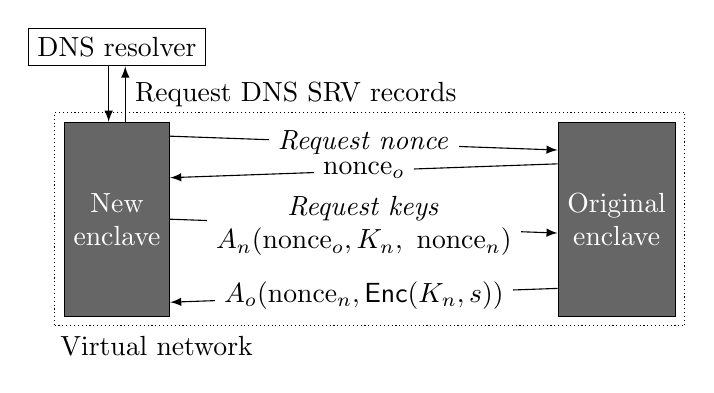
\begin{tikzpicture}[node distance=20pt]

  \node [draw,
         align=center,
         fill=black!20!gray,
         minimum height=70pt] (enclave2) {\color{white}New\\\color{white}enclave};
  \node [draw,
         align=center,
         fill=black!20!gray,
         minimum height=70pt,
         right=140pt of enclave2] (enclave1) {\color{white}Original\\\color{white}enclave};
  \node [draw,
         densely dotted,
         label=below left:Virtual network,
         fit=(enclave1) (enclave2)] {};

  \node [draw,
         above=of enclave2] (resolver) {DNS resolver};

  % New enclave discovers existing enclaves via DNS.
  \draw [-latex] ([xshift=3pt]enclave2.north) -- ([xshift=3pt]resolver.south)
        node [midway, right] {Request DNS SRV records};
  \draw [latex-] ([xshift=-3pt]enclave2.north) -- ([xshift=-3pt]resolver.south);

  % New enclave asks original enclave for nonce.
  \draw [-latex] ([yshift=30pt]enclave2.east) -- ([yshift=25pt]enclave1.west)
        node [midway, fill=white, align=center]
        {\emph{Request nonce}};
  \draw [latex-] ([yshift=15pt]enclave2.east) -- ([yshift=20pt]enclave1.west)
        node [midway, fill=white, align=center]
        {$\textrm{nonce}_o$};

  % New enclave asks for keys.
  \draw [-latex] (enclave2.east) -- ([yshift=-5pt]enclave1.west)
        node [midway, fill=white, align=center]
        {\emph{Request keys}\\$A_{n}(\textrm{nonce}_o, K_n, \ \textrm{nonce}_n$)};

  \draw [latex-] ([yshift=-30pt]enclave2.east) -- ([yshift=-25pt]enclave1.west)
        node [midway, fill=white, align=center]
        {$A_{o}(\textrm{nonce}_n, \textsf{Enc}(K_n, s))$};

\end{tikzpicture}

  \caption{When a new enclave bootstraps, it discovers existing enclaves by
    obtaining the DNS SRV record for its own, hard-coded FQDN.  The enclave then
    initiates key synchronization by first requesting a nonce.  Then, the new
    enclave requests the origin enclave's key material by submitting its own
    attestation document, followed by receiving the origin enclave's attestation
    document, which contains encrypted key material.}
  \label{fig:key-synchronization}
\end{figure}

\paragraph{First,} once a new enclave is spun up, it queries the DNS SRV record
of the FQDN that is hard-coded in the enclave, e.g., example.com.  The DNS
resolver will return the record, containing a list of enclaves that are already
running.  The new enclave picks a random enclave from the list and initiates
key synchronization.

\paragraph{Second,} the new enclave asks the existing enclave for a random
nonce, $\textrm{nonce}_o$.  The new enclave caches $\textrm{nonce}_o$ for one
minute.

\paragraph{Third,} the new enclave now requests the key material from the
existing enclave.  As part of the request, it provides its attestation document
that contains $\textrm{nonce}_o$ (to prove freshness to the existing enclave);
$\textrm{nonce}_n$ (the existing enclave is expected to add the nonce to its
attestation document); and $K_n$ (a public key to which the key material should
be encrypted).  Upon receipt of the new enclave's attestation document, the
existing enclave verifies the attestation document's signature and ensures that
the new enclave is running the same code, i.e., the PCR values are identical.
Once the new enclave is convinced that it is dealing with a genuine new
enclave, it creates an attestation document by including $\textrm{nonce}_n$ (to
prove freshness to the new enclave) and $\textsf{Enc}(K_n, s)$---the key
material $s$ is encrypted using the public key that the new enclave provided in
the request.  Finally, the new enclave verifies the attestation document,
decrypts the key material, and uses it to finish bootstrapping.

% Security considerations.
Needless to say, the security of key synchronization is critical.  The first
layer of defense is the fact that enclaves communicate with each other over a
virtual network that is part of a private Kubernetes cluster.  That means that
it's not possible for arbitrary Internet hosts to contact an enclave, and
request its key material.  The second layer of defense is the fact that an
enclave first has to provide a valid attestation document before obtaining key
material.  As long as an existing enclave knows that an identical and authentic
copy of itself is asking for key material, it will readily provide it.

\subsubsection{Thwarting Side-channel Attacks}
\label{sec:side-channels}

The enclave's parent EC2 image cannot see \emph{what} clients submit but it can
see \emph{how much} clients submit and \emph{how long} it takes the enclave to
process data.  The EC2 image can exploit these side channels to learn more
about the client's confidential information and computation.  While such side
channels must be avoided, our framework is not the place to do so.  Instead, it
is the application developer's responsibility to identify and address side
channels.  Section~\ref{sec:applications} introduces two applications and
discusses side channel attacks in their respective setting.

Similarly, programming bugs in the enclave application are also out of scope
for this work.  Memory corruption attacks me be more difficult to implement
against enclave applications\footnote{The untrustworthy operating system (that
may be under the attacker's control) is prohibited by hardware to read the
enclave application's memory or registers in clear text, which forces the
attacker to operate blindly.} but Lee et al. showed that it's possible, by
adapting a return-oriented programming attack against SGX~\cite{Lee2017a}.

\subsubsection{An Example}

Figure~\ref{fig:hello-world} illustrates an example of a simple ``hello world''
application.  The code initializes a new enclave struct (line 16), followed by
adding a handler that processes requests for \texttt{GET /hello-world} (line
24).  Finally, the application starts the enclave using a function call that
does not return (line 27).

\begin{figure}[t]
\begin{lstlisting}
package main

import (
    "fmt"
    "log"
    "net/http"

    nitro "REDACTED"
)

func handler(w http.ResponseWriter, r *http.Request) {
    fmt.Fprintln(w, "hello world")
}

func main() {
    enclave := nitro.NewEnclave(
        &nitro.Config{
            FQDN:    "example.com",
            Port:    8080,
            UseACME: true,
            Debug:   false,
        },
    )
    enclave.AddRoute(http.MethodGet,
                     "/hello-world",
                     handler)
    if err := enclave.Start(); err != nil {
        log.Fatalf("Terminated: %v", err)
    }
}
\end{lstlisting}
\caption{An example of a simple enclave application which registers an HTTP GET
  handler for the path /hello-world (line 24) and, when accessed, responds with
  the string ``hello world'' in the response body (line 12).}
\label{fig:hello-world}
\end{figure}

\section{Applications}
\label{sec:applications}

We demonstrate the practicality of our framework by building two applications on
to pof it.  First, in a novel system that pseudonymizes client IP addresses for
anti-fraud (\S~\ref{sec:pseudonymization}); second, to implement the shuffler
component that is part of Bittau et al.'s PROCHLO paper~\cite{Bittau2017a}
(\S~\ref{sec:shuffler}).  In both cases, we had to overcome minor obstacles but
found that our framework greatly facilitated the deployment of enclave code.

While our framework is written in Go, developers can build enclave applications
in languages other than Go, by taking advantage of a foreign function interface
(FFI) that allows Go code to invoke functions in other languages.  We
successfully moved a Rust code base into a Nitro enclave by implementing a
lightweight, Go-based wrapper (in less than 200 lines of code, excluding our
framework's code) that interacts with the Rust code via an FFI.\footnote{The
code is publicly available but we don't link to it yet to preserve our
anonymity.} Importantly, the compilation process is still reproducible as long
as the Rust code's dependencies are pinned via Rust's Cargo tool chain.

\subsection{IP Address Pseudonymizer}
\label{sec:pseudonymization}

Our first application is the system that originally motivated us to build the
enclave framework. Consider a service provider that offers various services to
its users.  The service provider seeks to know as little as possible about its
users, which means that it doesn't capture and store any of its users' IP
addresses.  IP addresses are however an important signal in the service
provider's fight against a subset of its users that commit fraud.  This
constitutes a conundrum: Should the service provider collect all its users' IP
addresses to strengthen its anti-fraud efforts?  Or continue to discard the
addresses, and tolerate the fraud?

This section presents an application that strikes a balance between these two
extremes; an IP address pseudonymization system that can verifiably pseudonymize
IP addresses.  The service provider can then run its anti-fraud logic over
pseudonymized IP addresses rather than real ones.  While some information is
lost in the process, we argue that what's most important---the relationship
between IP addresses---can be preserved thanks to our use of the Crypto-PAn
scheme that Xu et al. presented in their 2001 paper~\cite{Xu01a}.  Crypto-PAn
encrypts both IPv4 and IPv6 addresses by implementing a 1:1 mapping $f$ that is
keyed by $k$ from an IP address to its pseudonymized equivalent while
\emph{preserving the address's prefix}, i.e., two IP addresses that share an
$n$-bit prefix also share an $n$-bit prefix after pseudonymization as
illustrated by the following example:

\begin{align}
f(k, \textrm{``\underline{10.0.0.}1''})\phantom{23} = \textrm{``\underline{242.32.192.}193''} \\
f(k, \textrm{``\underline{10.0.0.}123''}) = \textrm{``\underline{242.32.192.}154''}
\end{align}

Figure~\ref{fig:address-anonymizer} illustrates the system design.  Clients
periodically communicate with a service behind a reverse TLS proxy whose
job---among other things---is to hide client IP addresses from the service.  The
proxy is configured to mirror incoming client requests to the enclave, but with
client IP addresses intact, in the form of a custom HTTP header like
\texttt{X-Client-Addr: 1.2.3.4}.  The service is interactive, and responds to
the client, but the enclave is passive, and simply consumes the requests.
Recall that the (untrusted) EC2 host that hosts the enclave is unable to see
the client's IP address because the TLS proxy establishes a TLS session that's
terminated \emph{inside} the enclave.  The pseudonymizer takes as input client
requests, extracts the IP address that the proxy inserted from the HTTP header,
pseudonymizes them, and forwards pseudonymized addresses in batches to the
configured back end.  Components in dark gray are under the service provider's
control.

\begin{figure}[t]
\centering
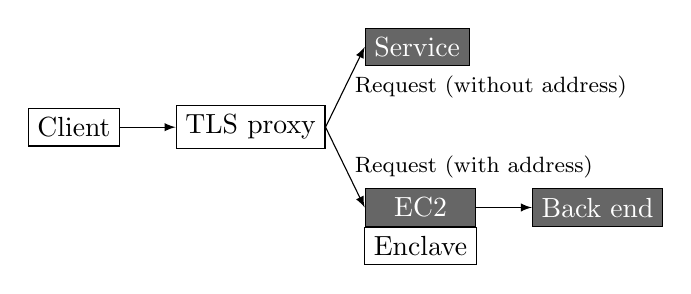
\begin{tikzpicture}[node distance=20pt]

\node [draw] (client) {Client};

\node [draw,
       right=of client] (proxy) {TLS proxy};

\node [draw,
       above right=of proxy,
       fill=black!20!gray] (service) {{\color{white} Service}};

\node [draw,
       fill=black!20!gray,
       minimum width=40pt,
       below right=of proxy] (ec2) {{\color{white} EC2}};

\node [draw,
       minimum width=40pt,
       below=0pt of ec2] (enclave) {Enclave};

\node [draw,
       right=of ec2,
       fill=black!20!gray] (backend) {{\color{white} Back end}};

\draw [-latex] (client.east) -- (proxy.west);

\draw [-latex] (proxy.east) -- (service.west)
      node [midway, right] {{\footnotesize Request (without address)}};

\draw [-latex] (proxy.east) -- (ec2.west)
      node [midway, right] {{\footnotesize Request (with address)}};

\draw [-latex] (ec2.east) -- (backend.west);

\end{tikzpicture}

\caption{Clients communicate with a service that's available behind a
  third-party TCP proxy whose purpose is (among other things) to drop client IP
  addresses, so the service never sees them.  The proxy is configured to mirror
  incoming client requests \emph{with} IP address to the enclave, where
  addresses are pseudonymized and finally forwarded to a back end for analysis.}
\label{fig:address-anonymizer}
\end{figure}

One problem however remains: how do clients know that the TLS proxy is in fact
configured to discard client IP addresses before forwarding requests to the
service?  Unfortunately, cloud providers don't offer satisfying solutions for
this problem but some cloud providers allow for the creation of roles whose
permissions are configurable.  The service provider can create a read-only role
in the TLS proxy's configuration interface and publish the credentials for this
role.  Doubtful users can then log in to this role and verify that the TLS proxy
is configured to discard IP addresses when forwarding requests to the service.
As long as the TLS proxy operator is a neutral third party with no incentive to
lie, which is typically the case, both the client and service provider can trust
it.  We acknowledge that this is not an elegant solution but a mere hack, to
work around the shortcoming of Nitro enclaves not having a networking interface.
If enclaves had a networking interface that could not be monitored by the
untrusted EC2 host, clients could directly talk to the enclave, obviating the
need for a TLS proxy that hides client IP addresses from the EC2 host.

\paragraph{Side channels}
The untrusted EC2 host never sees client IP address in plaintext
but it can exploit timing and volume side channels to infer information about
the encrypted requests that the TLS proxy forwards to the enclave.  We close
this side channel by adding code to the enclave application which queues
pseudonymized IP addresses until two conditions are true: (\emph{i}) we have at
least $n$ pseudonymized addresses, and (\emph{ii}) at least $t$ minutes have
passed.

\paragraph{Key rotation} A single pseudonymous IP address without context cannot
be reversed and reveals nothing about its corresponding plaintext IP address but
that changes if the service provider expects the client to repeatedly report its
IP address to the enclave.  For example, a sequence of pseudonymized IP
addresses can reveal either that (\emph{i}) the client has not changed its IP
address, or (\emph{ii}) the client changed its IP address but is likely to use
the same ISP (e.g., if the /24 prefix remains the same), or (\emph{iii}) the
client changed IP addresses \emph{and} ISPs (e.g., if the prefixes of the
pseudonymous IP addresses share less than, say, eight bits).  While this is
useful information for anti-fraud operations,\footnote{For example, a service
provider would deem a client that constantly changed ISPs suspicious; it is
likely to use proxies to connect to the service provider's infrastructure.} it
also reveals information about a given client's location, and service providers
may want to err on the side of privacy instead.  We therefore added a mechanism
for periodic key rotation, so a given client's pseudonymized IP addresses are
only meaningful within a given rotation period.  According to the results of
Padmanabhan et al., we believe that a key rotation period of three weeks strikes
a useful balance between privacy for the client and usefulness for the service
provider~\cite[\S~3.2]{Padmanabhan20a}: several ISPs re-assign many of their
users' IP addresses in less than---or up to---two weeks.

In the final step, the enclave submits the client's pseudonymized IP address and
a hash of the key to the service provider's back end, where anti-fraud logic is
implemented.  The implementation details of both the back end and its anti-fraud
logic are beyond the scope of this paper.

\paragraph{Implementation}
Our pseudonymization service counts approximately 1,000 lines of code, including
comments and tests.  It is important to keep the source code small for both
security and transparency: a large code base is more likely to have
security-critical bugs and is also more difficult for users to audit.

\paragraph{Alternative pseudonymization}
In addition to Crypto-PAn, we implemented a second pseudonymization method that
is based on HMAC-SHA-256.  Like Crypto-PAn, the HMAC is keyed by a 160-bit
secret that the enclave generates when first bootstrapping.  Unlike Crypto-PAn
however, the HMAC-based method does not preserve the prefixes of IP addresses:
two IP addresses that differ in only a single bit will result in entirely
different hashes.  On the privacy/utility spectrum, the HMAC-based method
therefore leans more toward privacy.

\subsection{$k$-anonymity Enforcer}
\label{sec:shuffler}

Bittau et al.'s SOSP'17 paper~\cite{Bittau2017a} proposes a private analytics
system that helps service providers gain insight into their clients' usage
patterns.  Their system---called PROCHLO---consists of three components:
(\emph{i}) software running on the client, which can (but doesn't have to) add
local differential privacy to client measurements.  Measurements consist of
product-relevant answers to questions like ``has the user interacted with her
browser in the last 24 hours?'' These measurements are then sent to (\emph{ii})
a shuffler, which enforces a configurable $k$-anonymity threshold on incoming
measurements.  The shuffler then sends measurements meeting that threshold to
(\emph{iii}) an analytics system that the service provider uses to explore
users' anonymized data.  The PROCHLO paper envisions the shuffler running in a
secure enclave; otherwise users would have no reason to trust that the shuffler
is in fact enforcing $k$-anonymity thresholds.  To that end, the authors
designed the shuffler to run inside an Intel SGX enclave, which was challenging
considering the memory constraints that SGX imposes.  For more details about the
shuffler, refer to the original PROCHLO paper~\cite[\S~3.3]{Bittau2017a}.

As part of an unrelated research project, we were experimenting with private
telemetry, and we therefore used our framework to re-implement the shuffler in
approximately 1,000 lines of code.\footnote{The code is freely available but we
omit a link to it to preserve our anonymity.}  Our implementation is a
near-complete clone of the shuffler as it was proposed in the PROCHLO paper but
for simplicity, we did not implement nested encryption~\cite[\S~3]{Bittau2017a}.
Figure~\ref{fig:shuffler} shows that our shuffler takes as input confidential
client measurements and enforces a configurable $k$-anonymity threshold on those
measurements.  Every $t$ seconds, the shuffler discards messages that don't meet
the threshold and forwards the remaining messages to its back end.\footnote{The
variable $t$ depends on the rate of incoming measurements.  Reasonable values
can range from hours (if the shuffler constantly sees a high rate of incoming
measurements) to days.} Before clients agree to sending their sensitive
measurements to the shuffler, they audit its source code and perform remote
attestation, to convince themselves that their measurements are processed by an
authentic enclave.

\begin{figure}[t]
\centering
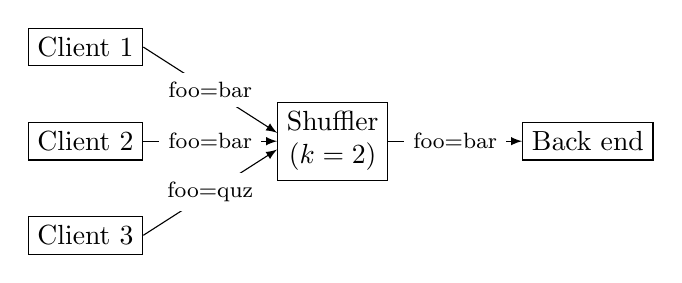
\begin{tikzpicture}[node distance=20pt]

\node [draw] (client1) {Client 1};
\node [draw, below=of client1] (client2) {Client 2};
\node [draw, below=of client2] (client3) {Client 3};

\node [draw, align=center, right=1.7 cm of client2] (shuffler) {Shuffler\\($k=2$)};
\node [draw, right=1.7 cm of shuffler] (backend) {Back end};

\draw [-latex] (client1.east) -- ([yshift=3pt]shuffler.west)
      node [midway, fill=white] {{\footnotesize foo=bar}};
\draw [-latex] (client2.east) -- (shuffler.west)
      node [midway, fill=white] {{\footnotesize foo=bar}};
\draw [-latex] (client3.east) -- ([yshift=-3pt]shuffler.west)
      node [midway, fill=white] {{\footnotesize foo=quz}};
\draw [-latex] (shuffler.east) -- (backend.west)
      node [midway, fill=white] {{\footnotesize foo=bar}};
nd) {Back end};

\end{tikzpicture}
\caption{A conceptual overview of our shuffler implementation.  Clients send
  measurements to the shuffler, which enforces a $k$-anonymity threshold---in
  this case for $k$=2. Only one of the two measurement types passes the
  threshold and is forwarded to the back end.}
\label{fig:shuffler}
\end{figure}

Compared to Bittau et al.'s original, SGX-based design, our Nitro-based
implementation has two key advantages: (\emph{i})~Nitro's underlying hardware
isolation makes our implementation more robust to hardware side channel attacks
and (\emph{ii})~Nitro doesn't suffer from the same resource constraints as SGX,
which renders our implementation easier to use and less error-prone.

\paragraph{Side channels}
The untrustworthy parent EC2 host can take advantage of the same side
channel as with the IP address pseudonymizer.  In particular, the EC2 host
can observe when and how many requests clients make.  Like with the IP address
pseudonymizer, the PROCHLO paper closes this side channel by aggregating
requests, preventing the EC2 host from linking incoming to outgoing
requests.

\section{Evaluation}
\label{sec:evaluation}

We evaluate our enclave framework with respect to
security (\S~\ref{sec:security}),
financial cost (\S~\ref{sec:cost}), and performance.  As for performance, we
study the rate at which one can generate
attestation documents (\S~\ref{sec:attestation-performance}) and
measure end-to-end request latency and throughput (\S~\ref{sec:end-to-end}).

\subsection{Security Considerations}
\label{sec:security}

There are three key components to the overall security of enclave applications;
(\emph{i}) Amazon's Nitro enclave system itself, (\emph{ii}) our framework, and
(\emph{iii}) the application that runs on top of our framework.

The very foundation of our framework's security lies in the soundness of the
design of Nitro enclaves.  While Amazon published the conceptual design, the
concrete hardware and software implementation remains confidential.  The
decision to allocate physically separate resources to enclaves appears promising
but only time will tell if Nitro enclaves can resist the types of attacks that
have been plagueing SGX.  If we assume that Nitro enclaves are acceptably
secure, the next critical layer is our software framework.

A significant security aspect of our framework is its size; it is well
understood that complexity is the enemy of security.  Our framework counts less
than 700 lines of code and has four direct dependencies that are not maintained
by either us or the Go project.\footnote{The dependencies are chi~\cite{chi}
(provides an HTTP request router), nsm~\cite{nsm} (provides an interface to
interact with the Nitro hypervisor), vsock~\cite{vsock} (provides an API for the
VSOCK address family), and tenus~\cite{tenus} (provides an API to configure
Linux's networking devices).}  Four is worse than zero, but is still manageable
and reasonably easy to audit in its entirety.  We believe that our choice of
using Go and the deliberately small trusted computing base greatly reduces---but
does not eliminate!---the attack surface.

The highest layer in the software stack is the enclave application itself.  The
biggest security threat are side channel attacks and programming bugs---both
unintentional and intentional.  It is the application developer's
responsibility to prevent side channel attacks and write bug-free code.  As we
pointed out in Section~\ref{sec:limitations}, programming bugs can be
intentional, i.e., the service provider may deliberately introduce bugs that
leak sensitive information.  From the user's point of view, eternal vigilance
is therefore the price of security.

\subsection{Financial Cost}
\label{sec:cost}

Nitro enclaves do not incur any extra cost in addition to what the underlying
EC2 host costs---they can be considered a ``free'' extension to EC2.  Nitro
enclaves are however only available for select types of EC2 instances because
they require their own CPU and a minimum amount of memory, and those instance
types are pricier than the lowest tier that AWS offers.

We are currently working on deploying the IP address pseudonymization prototype
that we introduced in Section~\ref{sec:pseudonymization}.  We estimate that our
enclave is going to have to handle an average of 5,000 requests per minute,
coming from more than ten million clients.  Our test deployment uses a single
c5.xlarge EC2 host in the U.S. East region which costs \$0.17 per hour to
operate, amounting to approximately \$125 per month.

\subsection{Attestation Documents}
\label{sec:attestation-performance}

The fetching of attestation documents is a critical part of our framework's
overall performance.  We wrote a stress test tool that requests as many
attestation documents as it can over sixty seconds.  The tool is essentially a
minimal enclave application that requests attestation documents in a loop.  For
each attestation document, we asked the hypervisor to include an incrementing
nonce, to avoid any speedups by caching.  We were able to obtain approximately
900 documents per second, with each request taking a median of one millisecond
($s = 0.3\,\text{ms}$) to fetch the attestation document.\footnote{We performed
our measurements on a c5.xlarge EC2 host which comes with four CPUs and eight
GiB of memory.}

\subsection{Application Latency and Throughput}
\label{sec:end-to-end}

Next, we set out to measure the networking latency of the critical path, as
illustrated in Figure~\ref{fig:stress-test}.  In particular, we test the
latency of our TCP proxy, the VSOCK interface between EC2 and enclave, and a
minimal enclave application.
%
We measure latency in three separate setups, designed to help us understand how
much latency each component in our data flow adds:

\begin{figure}[t]
    \centering
    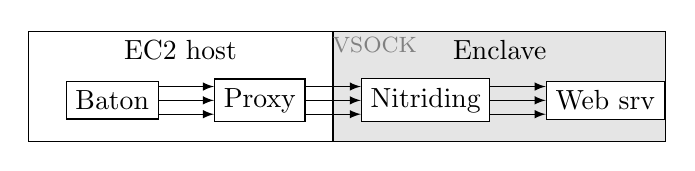
\begin{tikzpicture}[node distance=20pt]
  \node [draw,
         label={[anchor=north]above:EC2 host},
         minimum height=40pt,
         align=center,
         minimum width=110pt] (ec2) {};

  \node [draw,
         label={[anchor=north]above:Enclave},
         right=0pt of ec2,
         fill=black!10,
         minimum height=40pt,
         minimum width=120pt] (enclave) {};

  \node [draw,
         align=center,
         yshift=-5pt,
         left=10pt of ec2.east] (proxy) {Proxy};

  \node [draw,
         align=center,
         left=of proxy] (baton) {Baton};

  \node [draw,
         align=center,
         fill=white,
         yshift=-5pt,
         right=10pt of enclave.west] (nitriding) {Nitriding};

  \node [draw,
         align=center,
         fill=white,
         right=of nitriding] (app) {Web srv};

  \node [xshift=15pt,
         yshift=-5pt,
         align=center] at (enclave.north west)
    {\footnotesize \color{gray} VSOCK};

  % Baton talking to the Web service.
  \draw[-latex] ([yshift=5pt]baton.east) -- ([yshift=5pt]proxy.west);
  \draw[-latex] (baton.east) -- (proxy.west);
  \draw[-latex] ([yshift=-5pt]baton.east) -- ([yshift=-5pt]proxy.west);

  \draw[-latex] ([yshift=5pt]proxy.east) -- ([yshift=5pt]nitriding.west);
  \draw[-latex] (proxy.east) -- (nitriding.west);
  \draw[-latex] ([yshift=-5pt]proxy.east) -- ([yshift=-5pt]nitriding.west);

  \draw[-latex] ([yshift=5pt]nitriding.east) -- ([yshift=5pt]app.west);
  \draw[-latex] (nitriding.east) -- (app.west);
  \draw[-latex] ([yshift=-5pt]nitriding.east) -- ([yshift=-5pt]app.west);

\end{tikzpicture}

    \caption{Our stress test tool tests the performance of our critical path,
    consisting of the TCP proxy, the VSOCK interface, and Go's HTTP stack in
    the enclave application.}
    \label{fig:stress-test}
\end{figure}

\begin{description}
  \item[Full:] This represents the full data flow as it would occur in
    production, i.e. client $\rightarrow$ TCP proxy $\rightarrow$ VSOCK
    interface $\rightarrow$ enclave application.

  \item[No proxy:] This setup does not contain the TCP proxy, i.e., the client
    talks to the VSOCK interface directly, i.e. client $\rightarrow$ VSOCK
    interface $\rightarrow$ enclave application.

  \item[Direct:] This setup does not contain the TCP proxy and the VSOCK
    interface.  Instead, the client directly talks to an application instance that is
    running \emph{outside} the enclave, i.e., client $\rightarrow$ application.
\end{description}

As part of our measurement setup, We first deploy the code from
Figure~\ref{fig:hello-world}---a minimalistic application that responds with
the string ``hello world'' upon receiving requests for the path /hello-world.
It's important to use a minimalistic application because we're only interested
in the latency that is caused by the components \emph{before} a request reaches
the enclave application.

To simulate clients, we use the HTTP load test tool Baton~\cite{baton}.  We run
Baton on the parent EC2 host and instruct it to send as many requests to the
TCP proxy as possible within 30 seconds, using 50 concurrent threads.  We had to
patch Baton's source code to add VSOCK support (to be able to send requests
directly to the enclave via the VSOCK interface) and to log latency
percentiles.  Note that our measurements constitute a \emph{lower bound} of the
latency that is achievable.  Real-world applications will exhibit higher latency
because clients send their requests over the Internet (which adds considerable
networking latency) and the enclave application is likely to be more complex
(which adds computational latency).

Figure~\ref{fig:latency-msmts} illustrates the results for our three test
setups.  The full pipeline is able to sustain 7,500 requests per second, with a
mean latency of 12.7 milliseconds.  Removing the proxy nearly doubles the
requests to 14,100 per second and lowers the mean latency to 6.5.  Finally, a
direct connection to the application---without proxy and VSOCK interface--once
again nearly doubles the number of requests, reaching 27,900 per second, with a
mean latency of only 3.2 milliseconds.  Figure~\ref{fig:latency-cdf} shows the
empirical CDF of the same latency measurements for our three test setups.

\begin{figure}[t]
    \centering
    \begin{tabular}{l r r r}
    \toprule
      Setup & Reqs/sec & Mean lat. (ms) & Max lat. (ms) \\
    \midrule
    Full & 7,500 & 12.7 & 56.0 \\
    No proxy & 14,100 & 6.5 & 52.0 \\
    Direct & 27,900 & 3.2 & 50.0 \\
    \bottomrule
    \end{tabular}
    \caption{Using 100 concurrent requests and 100,000 requests in total.}
    \label{fig:latency-msmts}
\end{figure}


\begin{figure}[t]
    \centering
    % Created by tikzDevice version 0.12.3.1 on 2023-01-22 18:15:41
% !TEX encoding = UTF-8 Unicode
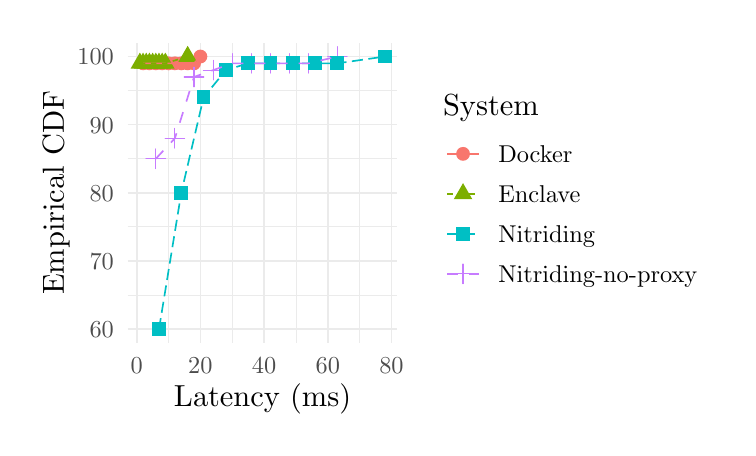
\begin{tikzpicture}[x=1pt,y=1pt]
\definecolor{fillColor}{RGB}{255,255,255}
\path[use as bounding box,fill=fillColor,fill opacity=0.00] (0,0) rectangle (252.94,144.54);
\begin{scope}
\path[clip] ( 36.11, 30.69) rectangle (133.59,139.04);
\definecolor{drawColor}{gray}{0.92}

\path[draw=drawColor,line width= 0.3pt,line join=round] ( 36.11, 47.92) --
	(133.59, 47.92);

\path[draw=drawColor,line width= 0.3pt,line join=round] ( 36.11, 72.55) --
	(133.59, 72.55);

\path[draw=drawColor,line width= 0.3pt,line join=round] ( 36.11, 97.18) --
	(133.59, 97.18);

\path[draw=drawColor,line width= 0.3pt,line join=round] ( 36.11,121.80) --
	(133.59,121.80);

\path[draw=drawColor,line width= 0.3pt,line join=round] ( 50.90, 30.69) --
	( 50.90,139.04);

\path[draw=drawColor,line width= 0.3pt,line join=round] ( 73.92, 30.69) --
	( 73.92,139.04);

\path[draw=drawColor,line width= 0.3pt,line join=round] ( 96.94, 30.69) --
	( 96.94,139.04);

\path[draw=drawColor,line width= 0.3pt,line join=round] (119.95, 30.69) --
	(119.95,139.04);

\path[draw=drawColor,line width= 0.6pt,line join=round] ( 36.11, 35.61) --
	(133.59, 35.61);

\path[draw=drawColor,line width= 0.6pt,line join=round] ( 36.11, 60.24) --
	(133.59, 60.24);

\path[draw=drawColor,line width= 0.6pt,line join=round] ( 36.11, 84.86) --
	(133.59, 84.86);

\path[draw=drawColor,line width= 0.6pt,line join=round] ( 36.11,109.49) --
	(133.59,109.49);

\path[draw=drawColor,line width= 0.6pt,line join=round] ( 36.11,134.11) --
	(133.59,134.11);

\path[draw=drawColor,line width= 0.6pt,line join=round] ( 39.39, 30.69) --
	( 39.39,139.04);

\path[draw=drawColor,line width= 0.6pt,line join=round] ( 62.41, 30.69) --
	( 62.41,139.04);

\path[draw=drawColor,line width= 0.6pt,line join=round] ( 85.43, 30.69) --
	( 85.43,139.04);

\path[draw=drawColor,line width= 0.6pt,line join=round] (108.45, 30.69) --
	(108.45,139.04);

\path[draw=drawColor,line width= 0.6pt,line join=round] (131.46, 30.69) --
	(131.46,139.04);
\definecolor{fillColor}{RGB}{248,118,109}

\path[fill=fillColor] ( 41.69,131.65) circle (  2.50);

\path[fill=fillColor] ( 43.99,131.65) circle (  2.50);

\path[fill=fillColor] ( 46.30,131.65) circle (  2.50);

\path[fill=fillColor] ( 48.60,131.65) circle (  2.50);

\path[fill=fillColor] ( 50.90,131.65) circle (  2.50);

\path[fill=fillColor] ( 53.20,131.65) circle (  2.50);

\path[fill=fillColor] ( 55.50,131.65) circle (  2.50);

\path[fill=fillColor] ( 57.81,131.65) circle (  2.50);

\path[fill=fillColor] ( 60.11,131.65) circle (  2.50);

\path[fill=fillColor] ( 62.41,134.11) circle (  2.50);
\definecolor{fillColor}{RGB}{124,174,0}

\path[fill=fillColor] ( 40.54,135.54) --
	( 43.91,129.71) --
	( 37.18,129.71) --
	cycle;

\path[fill=fillColor] ( 41.69,135.54) --
	( 45.06,129.71) --
	( 38.33,129.71) --
	cycle;

\path[fill=fillColor] ( 42.84,135.54) --
	( 46.21,129.71) --
	( 39.48,129.71) --
	cycle;

\path[fill=fillColor] ( 43.99,135.54) --
	( 47.36,129.71) --
	( 40.63,129.71) --
	cycle;

\path[fill=fillColor] ( 45.15,135.54) --
	( 48.51,129.71) --
	( 41.78,129.71) --
	cycle;

\path[fill=fillColor] ( 46.30,135.54) --
	( 49.66,129.71) --
	( 42.93,129.71) --
	cycle;

\path[fill=fillColor] ( 47.45,135.54) --
	( 50.81,129.71) --
	( 44.08,129.71) --
	cycle;

\path[fill=fillColor] ( 48.60,135.54) --
	( 51.96,129.71) --
	( 45.23,129.71) --
	cycle;

\path[fill=fillColor] ( 49.75,135.54) --
	( 53.11,129.71) --
	( 46.39,129.71) --
	cycle;

\path[fill=fillColor] ( 57.81,138.00) --
	( 61.17,132.17) --
	( 54.44,132.17) --
	cycle;
\definecolor{drawColor}{RGB}{199,124,255}

\path[draw=drawColor,line width= 0.4pt,line join=round,line cap=round] ( 42.76, 97.18) -- ( 49.83, 97.18);

\path[draw=drawColor,line width= 0.4pt,line join=round,line cap=round] ( 46.30, 93.64) -- ( 46.30,100.71);

\path[draw=drawColor,line width= 0.4pt,line join=round,line cap=round] ( 49.67,104.56) -- ( 56.73,104.56);

\path[draw=drawColor,line width= 0.4pt,line join=round,line cap=round] ( 53.20,101.03) -- ( 53.20,108.10);

\path[draw=drawColor,line width= 0.4pt,line join=round,line cap=round] ( 56.58,126.73) -- ( 63.64,126.73);

\path[draw=drawColor,line width= 0.4pt,line join=round,line cap=round] ( 60.11,123.19) -- ( 60.11,130.26);

\path[draw=drawColor,line width= 0.4pt,line join=round,line cap=round] ( 63.48,129.19) -- ( 70.55,129.19);

\path[draw=drawColor,line width= 0.4pt,line join=round,line cap=round] ( 67.01,125.66) -- ( 67.01,132.72);

\path[draw=drawColor,line width= 0.4pt,line join=round,line cap=round] ( 70.39,131.65) -- ( 77.45,131.65);

\path[draw=drawColor,line width= 0.4pt,line join=round,line cap=round] ( 73.92,128.12) -- ( 73.92,135.18);

\path[draw=drawColor,line width= 0.4pt,line join=round,line cap=round] ( 77.29,131.65) -- ( 84.36,131.65);

\path[draw=drawColor,line width= 0.4pt,line join=round,line cap=round] ( 80.82,128.12) -- ( 80.82,135.18);

\path[draw=drawColor,line width= 0.4pt,line join=round,line cap=round] ( 84.20,131.65) -- ( 91.26,131.65);

\path[draw=drawColor,line width= 0.4pt,line join=round,line cap=round] ( 87.73,128.12) -- ( 87.73,135.18);

\path[draw=drawColor,line width= 0.4pt,line join=round,line cap=round] ( 91.10,131.65) -- ( 98.17,131.65);

\path[draw=drawColor,line width= 0.4pt,line join=round,line cap=round] ( 94.63,128.12) -- ( 94.63,135.18);

\path[draw=drawColor,line width= 0.4pt,line join=round,line cap=round] ( 98.01,131.65) -- (105.07,131.65);

\path[draw=drawColor,line width= 0.4pt,line join=round,line cap=round] (101.54,128.12) -- (101.54,135.18);

\path[draw=drawColor,line width= 0.4pt,line join=round,line cap=round] (108.37,134.11) -- (115.43,134.11);

\path[draw=drawColor,line width= 0.4pt,line join=round,line cap=round] (111.90,130.58) -- (111.90,137.65);
\definecolor{fillColor}{RGB}{0,191,196}

\path[fill=fillColor] ( 44.95, 33.11) --
	( 49.95, 33.11) --
	( 49.95, 38.11) --
	( 44.95, 38.11) --
	cycle;

\path[fill=fillColor] ( 53.01, 82.37) --
	( 58.00, 82.37) --
	( 58.00, 87.36) --
	( 53.01, 87.36) --
	cycle;

\path[fill=fillColor] ( 61.06,116.84) --
	( 66.06,116.84) --
	( 66.06,121.84) --
	( 61.06,121.84) --
	cycle;

\path[fill=fillColor] ( 69.12,126.69) --
	( 74.11,126.69) --
	( 74.11,131.69) --
	( 69.12,131.69) --
	cycle;

\path[fill=fillColor] ( 77.18,129.15) --
	( 82.17,129.15) --
	( 82.17,134.15) --
	( 77.18,134.15) --
	cycle;

\path[fill=fillColor] ( 85.23,129.15) --
	( 90.23,129.15) --
	( 90.23,134.15) --
	( 85.23,134.15) --
	cycle;

\path[fill=fillColor] ( 93.29,129.15) --
	( 98.28,129.15) --
	( 98.28,134.15) --
	( 93.29,134.15) --
	cycle;

\path[fill=fillColor] (101.34,129.15) --
	(106.34,129.15) --
	(106.34,134.15) --
	(101.34,134.15) --
	cycle;

\path[fill=fillColor] (109.40,129.15) --
	(114.40,129.15) --
	(114.40,134.15) --
	(109.40,134.15) --
	cycle;

\path[fill=fillColor] (126.66,131.62) --
	(131.66,131.62) --
	(131.66,136.61) --
	(126.66,136.61) --
	cycle;
\definecolor{drawColor}{RGB}{248,118,109}

\path[draw=drawColor,line width= 0.6pt,line join=round] ( 41.69,131.65) --
	( 43.99,131.65) --
	( 46.30,131.65) --
	( 48.60,131.65) --
	( 50.90,131.65) --
	( 53.20,131.65) --
	( 55.50,131.65) --
	( 57.81,131.65) --
	( 60.11,131.65) --
	( 62.41,134.11);
\definecolor{drawColor}{RGB}{124,174,0}

\path[draw=drawColor,line width= 0.6pt,dash pattern=on 2pt off 2pt ,line join=round] ( 40.54,131.65) --
	( 41.69,131.65) --
	( 42.84,131.65) --
	( 43.99,131.65) --
	( 45.15,131.65) --
	( 46.30,131.65) --
	( 47.45,131.65) --
	( 48.60,131.65) --
	( 49.75,131.65) --
	( 57.81,134.11);
\definecolor{drawColor}{RGB}{0,191,196}

\path[draw=drawColor,line width= 0.6pt,dash pattern=on 4pt off 2pt ,line join=round] ( 47.45, 35.61) --
	( 55.50, 84.86) --
	( 63.56,119.34) --
	( 71.62,129.19) --
	( 79.67,131.65) --
	( 87.73,131.65) --
	( 95.79,131.65) --
	(103.84,131.65) --
	(111.90,131.65) --
	(129.16,134.11);
\definecolor{drawColor}{RGB}{199,124,255}

\path[draw=drawColor,line width= 0.6pt,dash pattern=on 4pt off 4pt ,line join=round] ( 46.30, 97.18) --
	( 53.20,104.56) --
	( 60.11,126.73) --
	( 67.01,129.19) --
	( 73.92,131.65) --
	( 80.82,131.65) --
	( 87.73,131.65) --
	( 94.63,131.65) --
	(101.54,131.65) --
	(111.90,134.11);
\end{scope}
\begin{scope}
\path[clip] (  0.00,  0.00) rectangle (252.94,144.54);
\definecolor{drawColor}{gray}{0.30}

\node[text=drawColor,anchor=base east,inner sep=0pt, outer sep=0pt, scale=  0.88] at ( 31.16, 32.58) {60};

\node[text=drawColor,anchor=base east,inner sep=0pt, outer sep=0pt, scale=  0.88] at ( 31.16, 57.21) {70};

\node[text=drawColor,anchor=base east,inner sep=0pt, outer sep=0pt, scale=  0.88] at ( 31.16, 81.83) {80};

\node[text=drawColor,anchor=base east,inner sep=0pt, outer sep=0pt, scale=  0.88] at ( 31.16,106.46) {90};

\node[text=drawColor,anchor=base east,inner sep=0pt, outer sep=0pt, scale=  0.88] at ( 31.16,131.08) {100};
\end{scope}
\begin{scope}
\path[clip] (  0.00,  0.00) rectangle (252.94,144.54);
\definecolor{drawColor}{gray}{0.30}

\node[text=drawColor,anchor=base,inner sep=0pt, outer sep=0pt, scale=  0.88] at ( 39.39, 19.68) {0};

\node[text=drawColor,anchor=base,inner sep=0pt, outer sep=0pt, scale=  0.88] at ( 62.41, 19.68) {20};

\node[text=drawColor,anchor=base,inner sep=0pt, outer sep=0pt, scale=  0.88] at ( 85.43, 19.68) {40};

\node[text=drawColor,anchor=base,inner sep=0pt, outer sep=0pt, scale=  0.88] at (108.45, 19.68) {60};

\node[text=drawColor,anchor=base,inner sep=0pt, outer sep=0pt, scale=  0.88] at (131.46, 19.68) {80};
\end{scope}
\begin{scope}
\path[clip] (  0.00,  0.00) rectangle (252.94,144.54);
\definecolor{drawColor}{RGB}{0,0,0}

\node[text=drawColor,anchor=base,inner sep=0pt, outer sep=0pt, scale=  1.10] at ( 84.85,  7.64) {Latency (ms)};
\end{scope}
\begin{scope}
\path[clip] (  0.00,  0.00) rectangle (252.94,144.54);
\definecolor{drawColor}{RGB}{0,0,0}

\node[text=drawColor,rotate= 90.00,anchor=base,inner sep=0pt, outer sep=0pt, scale=  1.10] at ( 13.08, 84.86) {Empirical CDF};
\end{scope}
\begin{scope}
\path[clip] (  0.00,  0.00) rectangle (252.94,144.54);
\definecolor{drawColor}{RGB}{0,0,0}

\node[text=drawColor,anchor=base west,inner sep=0pt, outer sep=0pt, scale=  1.10] at (150.09,112.73) {System};
\end{scope}
\begin{scope}
\path[clip] (  0.00,  0.00) rectangle (252.94,144.54);
\definecolor{fillColor}{RGB}{248,118,109}

\path[fill=fillColor] (157.32, 98.94) circle (  2.50);
\end{scope}
\begin{scope}
\path[clip] (  0.00,  0.00) rectangle (252.94,144.54);
\definecolor{drawColor}{RGB}{248,118,109}

\path[draw=drawColor,line width= 0.6pt,line join=round] (151.54, 98.94) -- (163.10, 98.94);
\end{scope}
\begin{scope}
\path[clip] (  0.00,  0.00) rectangle (252.94,144.54);
\definecolor{fillColor}{RGB}{124,174,0}

\path[fill=fillColor] (157.32, 88.37) --
	(160.68, 82.54) --
	(153.96, 82.54) --
	cycle;
\end{scope}
\begin{scope}
\path[clip] (  0.00,  0.00) rectangle (252.94,144.54);
\definecolor{drawColor}{RGB}{124,174,0}

\path[draw=drawColor,line width= 0.6pt,dash pattern=on 2pt off 2pt ,line join=round] (151.54, 84.48) -- (163.10, 84.48);
\end{scope}
\begin{scope}
\path[clip] (  0.00,  0.00) rectangle (252.94,144.54);
\definecolor{fillColor}{RGB}{0,191,196}

\path[fill=fillColor] (154.82, 67.53) --
	(159.82, 67.53) --
	(159.82, 72.53) --
	(154.82, 72.53) --
	cycle;
\end{scope}
\begin{scope}
\path[clip] (  0.00,  0.00) rectangle (252.94,144.54);
\definecolor{drawColor}{RGB}{0,191,196}

\path[draw=drawColor,line width= 0.6pt,dash pattern=on 4pt off 2pt ,line join=round] (151.54, 70.03) -- (163.10, 70.03);
\end{scope}
\begin{scope}
\path[clip] (  0.00,  0.00) rectangle (252.94,144.54);
\definecolor{drawColor}{RGB}{199,124,255}

\path[draw=drawColor,line width= 0.4pt,line join=round,line cap=round] (153.79, 55.57) -- (160.85, 55.57);

\path[draw=drawColor,line width= 0.4pt,line join=round,line cap=round] (157.32, 52.04) -- (157.32, 59.11);
\end{scope}
\begin{scope}
\path[clip] (  0.00,  0.00) rectangle (252.94,144.54);
\definecolor{drawColor}{RGB}{199,124,255}

\path[draw=drawColor,line width= 0.6pt,dash pattern=on 4pt off 4pt ,line join=round] (151.54, 55.57) -- (163.10, 55.57);
\end{scope}
\begin{scope}
\path[clip] (  0.00,  0.00) rectangle (252.94,144.54);
\definecolor{drawColor}{RGB}{0,0,0}

\node[text=drawColor,anchor=base west,inner sep=0pt, outer sep=0pt, scale=  0.88] at (170.05, 95.91) {Docker};
\end{scope}
\begin{scope}
\path[clip] (  0.00,  0.00) rectangle (252.94,144.54);
\definecolor{drawColor}{RGB}{0,0,0}

\node[text=drawColor,anchor=base west,inner sep=0pt, outer sep=0pt, scale=  0.88] at (170.05, 81.45) {Enclave};
\end{scope}
\begin{scope}
\path[clip] (  0.00,  0.00) rectangle (252.94,144.54);
\definecolor{drawColor}{RGB}{0,0,0}

\node[text=drawColor,anchor=base west,inner sep=0pt, outer sep=0pt, scale=  0.88] at (170.05, 67.00) {Nitriding};
\end{scope}
\begin{scope}
\path[clip] (  0.00,  0.00) rectangle (252.94,144.54);
\definecolor{drawColor}{RGB}{0,0,0}

\node[text=drawColor,anchor=base west,inner sep=0pt, outer sep=0pt, scale=  0.88] at (170.05, 52.54) {Nitriding-no-proxy};
\end{scope}
\end{tikzpicture}

    \label{fig:latency-cdf}
    \caption{The empirical CDF of the latency distributions of our three test setups.}
\end{figure}

Next, we measure the throughput that we can achieve over the VSOCK interface.
To that end, we use a VSOCK-enabled fork of the iperf3 performance measurement
tool~\cite{iperf-vsock}.  iperf3 measures the throughput of a networking link
using a client/server model.  In our experiment, we start an iperf3 server
instance inside the enclave and the corresponding client instance on the parent
EC2 host.\footnote{The command that we ran on the server was
``\texttt{iperf3 -{}-vsock -s}'' and on the client ``\texttt{iperf3 -{}-vsock -c
4}.''} The client then talks to the server via the VSOCK interface and
determines the maximum possible throughput.  In this setup, iperf3 measured a
throughput of 4.09 GBit/s.  For comparison, when running both the iperf3 client
\emph{and} server on the EC2 host---which effectively measures the
throughput of the EC2 host's loopback interface---we achieve 55.5 GBit/s of
throughput.

To develop intuition on the perceived network performance of Nitro enclaves, we
built an enclave application that acts as a SOCKS proxy.  We then configured a
browser to use this enclave-enabled SOCKS proxy and browsed HD videos on
YouTube.  We found that the experience was seamless: videos loaded quickly,
played smoothly, and there was no perceivable latency impact when browsing the
Web.  We believe that the high throughput and low latency, coupled with this
anecdotal user experience report suggests that our framework is suitable for
demanding and latency-sensitive networking applications.

% \subsection{Operational Experience}
% \label{sec:operations}
%
%
% \begin{itemize}
%     \item We deployed application X on YYYY-MM-DD.
%
%     \item How many clients were involved?  How many requests per second did
%     they make?
%
%     \item We published a blog post.  Discuss user reception.
%
%     \item Discuss how useful we found the system in the context of
%     anti-fraud.
%
%     \item Discuss operational issues and gotchas.
% \end{itemize}

\section{Limitations}%
\label{sec:limitations}

We conclude the discussion of our framework by summarizing its limitations.

% Everybody needs to trust Amazon.
An obvious limitation is the reliance of our framework on Amazon, which acts as
the root of trust.  We mentioned in Section~\ref{sec:assumptions-overview} that
all parties must trust Amazon.  Note that this is not a new limitation of secure
enclaves---SGX-based applications must trust Intel while TrustZone-based
applications must trust ARM.  Despite the lack of alternatives, placing one's
trust in a single corporation's proprietary technology is problematic.

% Laypeople cannot audit enclave code.
Our system fundamentally relies on at least some users auditing the service
provider's application that runs in a secure enclave.  Needless to say, not all
users have the skills to audit the service provider's application and convince
themselves that the code is sound.  In fact, even among the subset of users that
are programmers, only a fraction may feel comfortable auditing source code for
vulnerabilities.  So what are the non-programmers to do?  We envision users to
congregate in forums where matters related to the service providers are
discussed.  A tech-savvy subset of the users is going to organize code reviews
and make public their findings.  Non-technical users may then trust other users
that audited the source code, but this is no different from most other software:
nobody audits all the software that they use, ranging from the kernel to the
myriad of user space applications, even when source code is available.

% One can hide bugs in plain sight.
The Underhanded C Coding Contest~\cite{underhanded-c} was about implementing
benign-looking code that was secretly malicious.  The contest attracted numerous
impressive submissions which showed that it can be surprisingly difficult to
find bugs \emph{even if one knows} that there is a bug in a given piece of code.
Analogously, the service provider could try to hide subtle, yet critical bugs in
the code to exfiltrate information from the enclave.  On top of that, if the
service provider ever gets caught, it may have plausible deniability and pretend
that the exfiltration bug was an honest programming error.  While we are unable
to solve this class of attacks, we can mitigate it by keeping the trusted
computing base in the enclave as small as possible.

\section{Related Work}
\label{sec:related-work}

\begin{itemize}
    \item https://openenclave.io/sdk/
    \item Project Oak
    \item Google Asylo
\end{itemize}

Lee et al. propose Keystone in their EuroSys'20 paper~\cite{Lee2020a}---an open
framework for the construction of secure enclaves based on the RISC-V
instruction set.  Keystone is customizable, open source, and based on commodity
hardware.

Work is similar to privacy-preserving analytics (PROCHLO/RAPPOR) but differs in the sense that clients have an incentive to lie, and we therefore cannot trust their reports.

\subsection{IP Address *nymization}

% How is our work different from traffic trace anonymization.

In their 2006 CCR article, Pang et al. summarize their experience in obtaining permission to publish packet traces, implementing the anonymization policy, and demonstrating its correctness~\cite{Pang06a}.

Difficult to anonymize traces~\cite{Burkhart10a}. Trade-off~\cite{Mohammady15a}

\subsection{Applications of Secure Enclaves}

Researchers have proposed numerous and diverse enclave-enabled systems, ranging from DeFi oracles~\cite{Zhang16a}, to health apps for COVID-19~\cite{Mailthody21a}, to networking middleboxes~\cite{Han17a}.

Despite avid interest in academia, real-world deployments of enclaves are sparse.  In 2017, the Signal secure messenger published a blog post on private contact discovery~\cite{Marlinspike17a}, which makes it possible for Alice to discover which of the contacts in her address book use Signal without revealing her contact list.  The Signal team accomplished this by relying on an SGX enclave that runs the contact discovery code.  Two years later, in 2019, the Signal team built its ``secure value recovery'' feature on SGX as well~\cite{Lund19a}.

\subsection{Attacks Against Secure Enclaves}

https://sgaxe.com/files/SGAxe.pdf

\textsc{Foreshadow}~\cite{Bulck18a}
\cite{Bulck19a}


Nilsson et al. surveyed existing SGX attacks in a 2020 arXiv report~\cite{Nilsson20a}.

\subsection{Libraries}

Open Enclave SDK provides an SDK for C and C++ that facilitates enclave development for SGX and TrustZone.
https://github.com/openenclave/openenclave


\balance
\printbibliography

\end{document}
